\documentclass{beamer}

\usepackage[czech]{babel}
\usepackage[utf8]{inputenc}
%\usepackage[plainpages=false,pdfpagelabels,unicode]{hyperref}
\usepackage{graphicx}
\usepackage{pdfpages}
\usepackage{color}

%\usepackage{biblatex}
%\addbibresource{bib-db.bib}

\usetheme{Warsaw}

\begin{document}

\title[Optical properties of HfO$_2$] % (optional, only for long titles)
{Optical properties of HfO$_2$ from first principles}
\subtitle{Short summary}
\author{Pavel Ondračka, David Holec}
\institute
{
	 Faculty of Science, Masaryk University\\
	Brno, Czech Republic
  \and
	CEITEC - Central European Institute of Technology\\
	Brno, Czech Republic
   \and 
   Department of Physical Metallurgy and Materials Testing\\
   Montanuniversität Leoben, Leoben, Austria
}
\date{23.06.2015}

\maketitle

\begin{frame}
	\frametitle{Outline}
    \tableofcontents
\end{frame}

\section{Motivation}


\begin{frame}
\frametitle{Motivation}
\framesubtitle{Why is HfO$_2$ cool}

\begin{itemize}
   \item HfO 2 is attracting a lot of attention as a high-k material
for electronic applications as well as optical applications
such as antireflective coatings, heat-mirrors, or laser mirrors.
   \item Quite simple benchmark system.
   \item Lot of experimental data available.
   \item Dispersion models available, can be further improved by calculations.
\end{itemize}
\end{frame}


\section{Methodology}


\begin{frame}
   \frametitle{Methodology}
\begin{itemize}
   \item VASP pseudopotential code used for structural relaxation and amorphous cells generation
   \item Wien2k full potential all electron code used for calculation of optical properties
   \item standard PBE used for structural properties, TB-mBJ used for optical stuff
   \item ,,simulated annealing'' procedure for generation or amorphous cells
   \item dielectric function calculated using the independent particles approximation (no excitons)
   \item 0\,K temperature (no phonons and indirect transitions)
\end{itemize}

\end{frame}

\section{Results}

\subsection{Band gaps}
\begin{frame}
    \frametitle{HfO$_2$ band gaps}
   

   \begin{table}
   \begin{center}
   \scriptsize
   \begin{tabular}{c|ccccc}
			   & TB-mBJ & PBE & hybrid funkcionals & GW$_0$ & experiment \\
   \hline
   m-HfO$_2$ &	5.75 & 4.08 & PBE0: 6.75, HSE06: 5.98 & 5.9 & 5.68 \\
   c-HfO$_2$ &	5.88 & 3.77 & SX: 5.6, HSE06: 5.38 & 5.5 & 5.8\\
   t-HfO$_2$ &	6.64 & 4.79 &  & 6.0 & \\
   am-HfO$_2$ & \color{red}5.53, 5.65 & & \color{black} PBE0: 5.3, 5.94 &  & 5.49--5.72, 5.62\\

   \end{tabular}
   \end{center}
   \end{table}


\begin{itemize}
   \item nearly perfect agreement with experiment
   \item in line with much more sophisticated hybrid and GW$_0$ approaches
   \item problems with calculated amorphous band gap
\end{itemize}


\end{frame}


\subsection{Dielectric functions}
\begin{frame}
    \frametitle{HfO$_2$ dielectric function}

	\begin{columns}[c]
    \column{.8\textwidth}
	\vspace{-0.5cm}

    \begin{figure}
	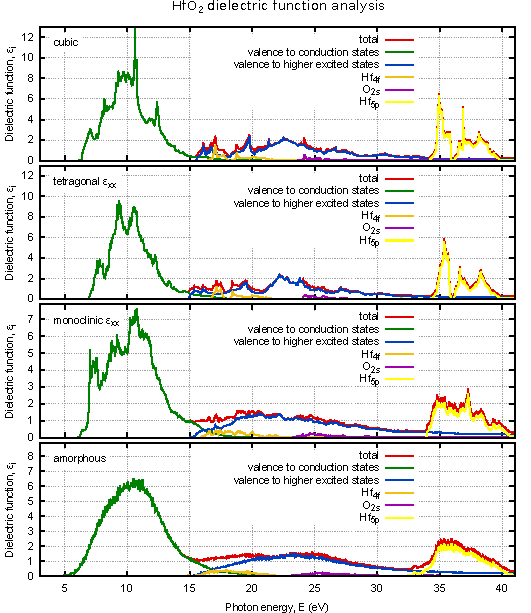
\includegraphics[height=6.8cm]{figures/cubic-eps.pdf}
	\end{figure}

    \column{.2\textwidth}
	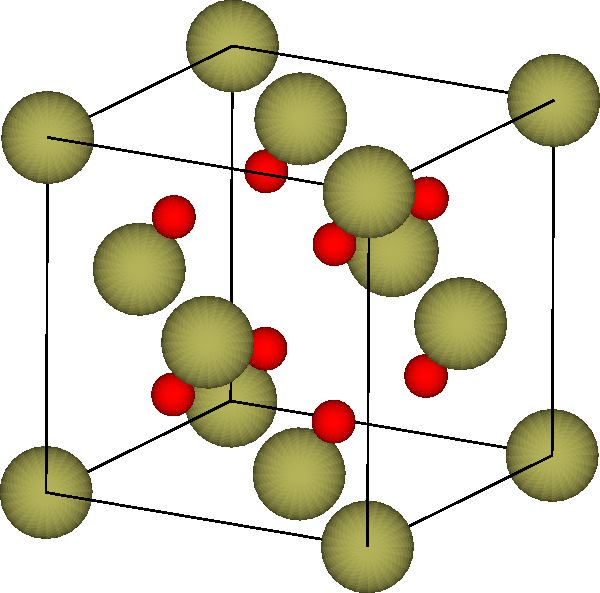
\includegraphics[width=0.75\linewidth]{figures/cubic.pdf}

	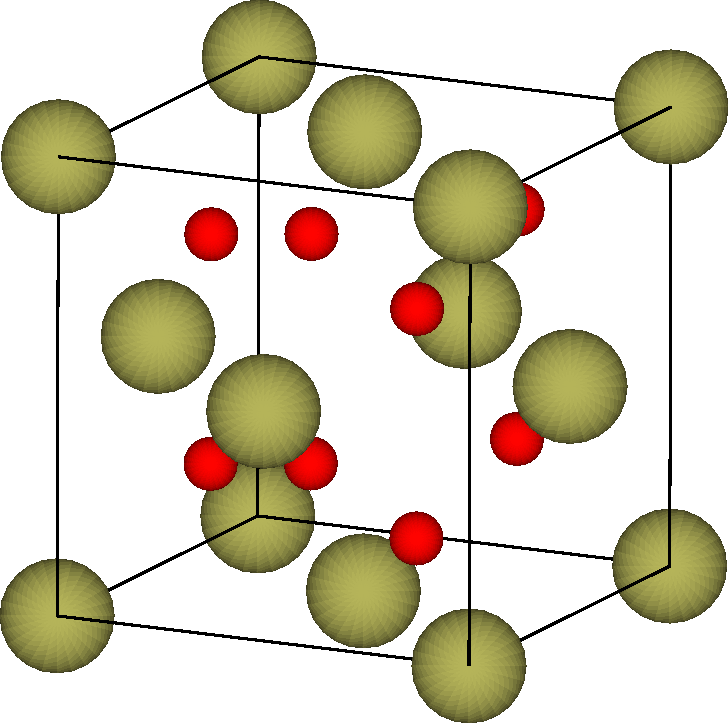
\includegraphics[width=0.75\linewidth]{figures/tetragonal.pdf}

	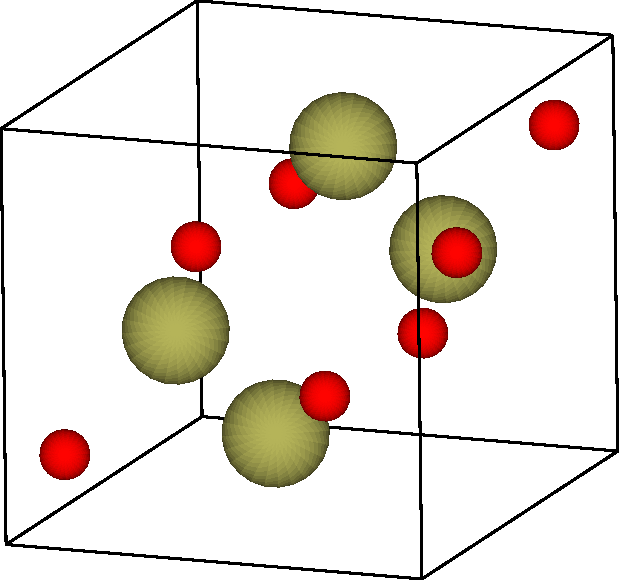
\includegraphics[width=0.75\linewidth]{figures/monoclinic.pdf}

	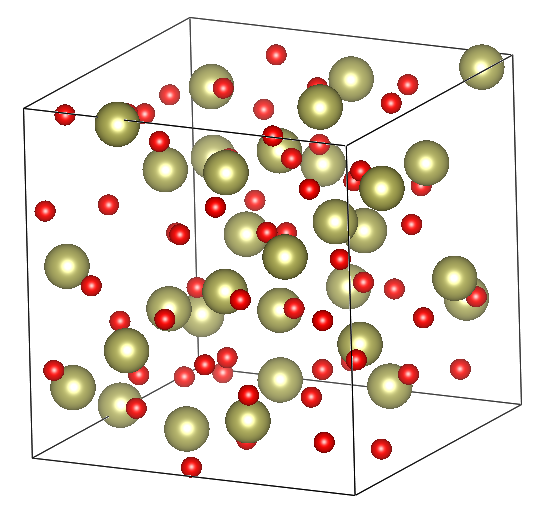
\includegraphics[width=0.75\linewidth]{figures/am.png}
    \end{columns}

\end{frame}


\begin{frame}
    \frametitle{Comparison with experiment}

	\begin{columns}[c]
    \column{.5\textwidth}
	\pause
   \vspace{-0.5cm}

    \begin{figure}
	\includegraphics[width=\linewidth]{figures/m-HfO2.pdf}
	\end{figure}

   \pause
   \vspace{-0.7cm}

    \begin{figure}
	\includegraphics[width=\linewidth]{figures/c-HfO2.pdf}
	\end{figure}
   \vspace{-0.5cm}

    \column{.5\textwidth}

   \pause

    \begin{figure}
	\includegraphics[width=\linewidth]{figures/am-HfO2.pdf}
	\end{figure}

   Not looking so good anymore...  

    \end{columns}

\end{frame}


\begin{frame}
    \frametitle{Origin of the discrepancy}
    \framesubtitle{too many approximations}

   \begin{center}
   	\includegraphics[width=0.6\linewidth]{figures/m-HfO2-hf.pdf}
   \end{center}

   Orders of magnitude more computational expensive hybrid functional doesn't offer any improvement.

\end{frame}


\subsection{Structural VS optical properties}

\begin{frame}
    \frametitle{Structural properties of HfO$_2$}
   \vspace{-0.4cm}
         \begin{figure}
	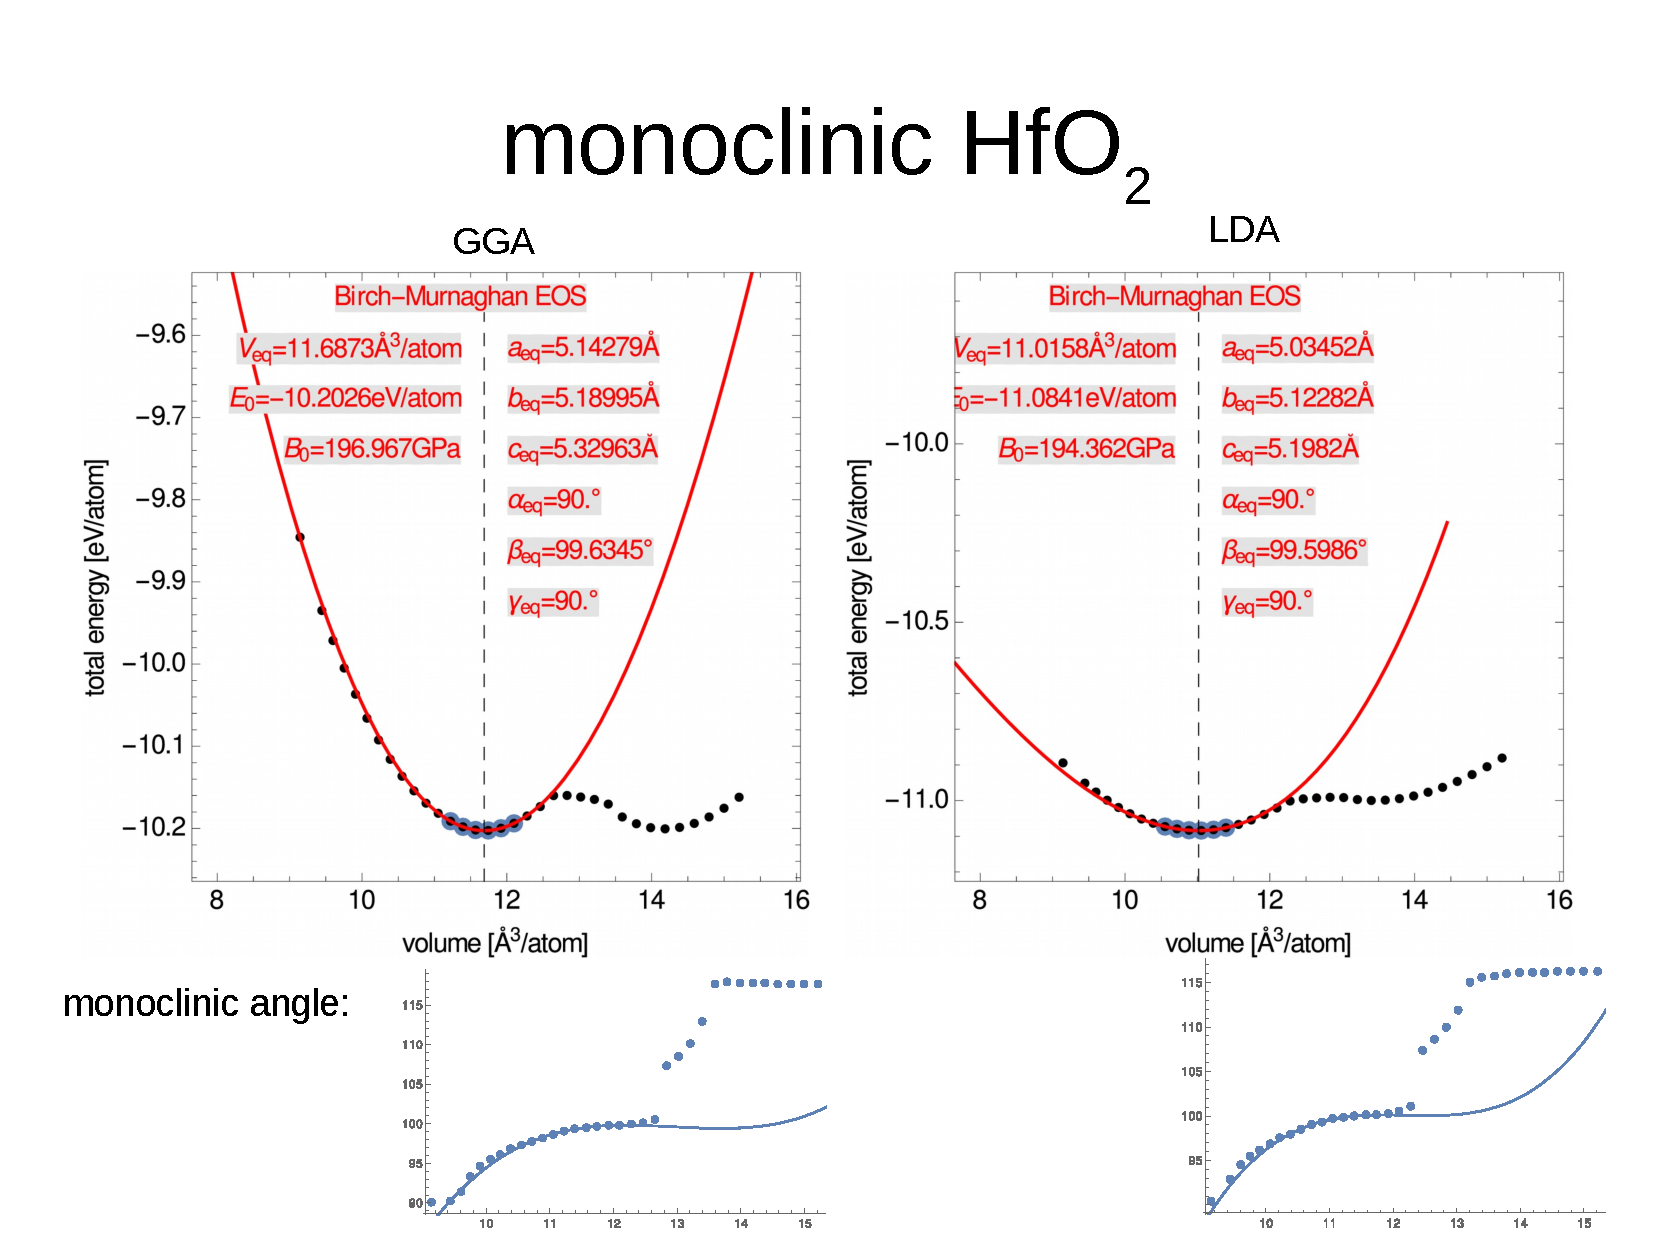
\includegraphics[width=0.9\linewidth]{figures/HfO2-monoclinic.pdf}
	\end{figure} 
\end{frame}

\begin{frame}
    \frametitle{Cell relaxation effect}
	\begin{columns}
	\begin{column}{0.4\linewidth}
		\begin{itemize}
			\item Residual forces are unphysical and unwanted
			\item Hugely affects all properties (like a band gap)
			\item Different relaxation procedures have slightly different results
		\end{itemize}
	\end{column}
	\begin{column}{0.6\linewidth}
		\includegraphics[width=\linewidth]{figures/gap.pdf}
	\end{column}
	\end{columns}

\end{frame}

\begin{frame}
    \frametitle{Effect of cell stress on band gap}
	\begin{columns}
	\begin{column}{0.4\linewidth}
		\begin{itemize}
			\item only preliminary results 
			\item significant dependence observed
		\end{itemize}
	\end{column}
	\begin{column}{0.6\linewidth}
		\includegraphics[width=\linewidth]{figures/V-gap.pdf}
	\end{column}
	\end{columns}
\end{frame}

\section{Conclusion}
\begin{frame}
		\begin{itemize}
			\item we can predict HfO$_2$ band gaps with high accuracy
			\item how to interpret and compare gap in amorphous materials is not clear yet
         \item calculated dielectric function underestimated
         \item hopefully this can be solved by adding excitonic effects
         \item interesting structural properties discovered, including band gap stress dependence
		\end{itemize}

      Thank you for your attention.
 
\end{frame}

\end{document}
